\chapter{Introduction à la science des robots manipulateurs}

La première partie de ces notes discute de la science pour modéliser et analyser le mouvement des robots manipulateurs. Dans un contexte d'ingénierie, modéliser un système robotique est essentiel lors de la phase de conception, par exemple pour valider qu'une géométrie de bras permet d'atteindre plusieurs positions désirées avec son effecteur (i.e. l'outil au bout du bras), et aussi lors de la programmation pour coordonner les différents moteurs et articulations d'un robot. Les outils présentés dans ces notes sont pertinents pour les mécanismes avec plusieurs articulations, on parlera toutefois de \textit{robot} pour alléger le texte.

\video{Introduction à l'analyse des robots manipulateurs}{https://youtu.be/N9cYzmWeyKM}

Comme illustré à la figure \ref{fig:fields}, la modélisation des robots peut être séparée en quatre grandes familles d'analyse.

%%%%%%%%%%%%%%%%%%%%%%%%%%%%%%%%%%%%%%%%%%%%%%%%%%%%%%%%%%%%%%%%%%%%%%%%%%%%%
\begin{figure}[H]
	\centering
		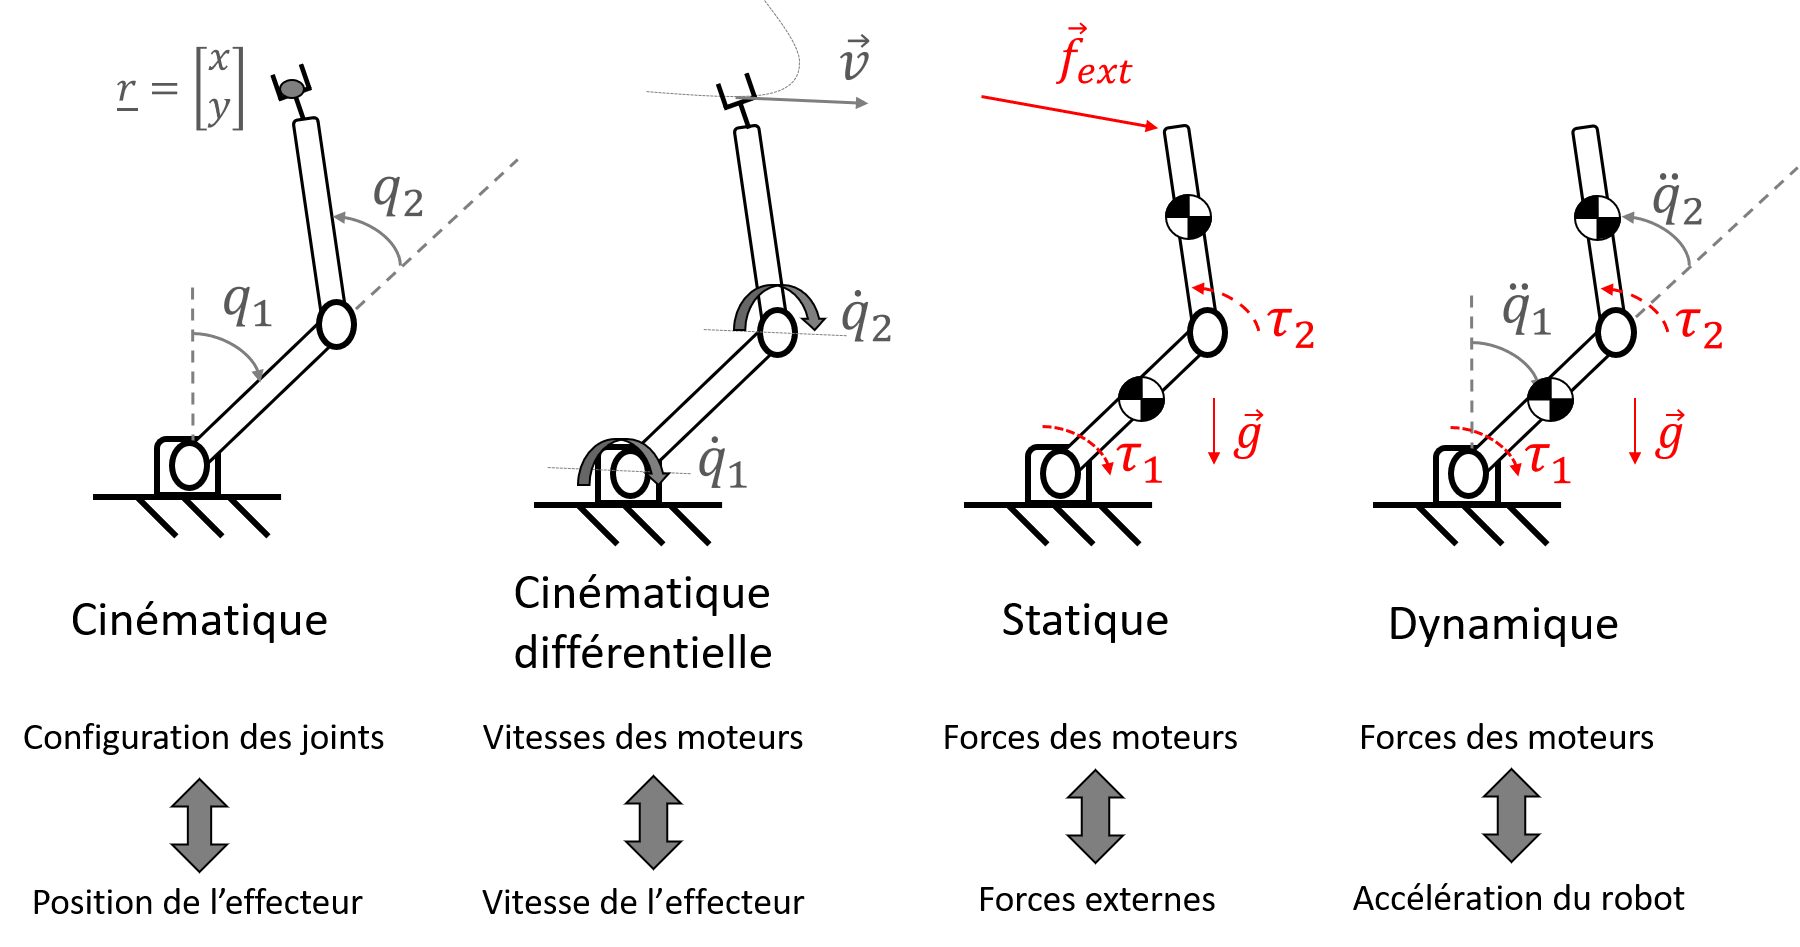
\includegraphics[width=0.90\textwidth]{fields.png}
	\caption{Quatre grands domaines de base de l'analyse de robots manipulateurs  }
	\label{fig:fields}
\end{figure}
%%%%%%%%%%%%%%%%%%%%%%%%%%%%%%%%%%%%%%%%%%%%%%%%%%%%%%%%%%%%%%%%%%%%%%%%%%%%%%%

Les méthodes de \textbf{cinématique directe} visent à calculer la position finale de l'effecteur d'un robot en fonction du positionnement des articulations. Lorsqu'on parle de \textbf{cinématique inverse}, l'objectif est de déterminer le positionnement des articulations qui mène à une position désirée de l'effecteur du robot. Mathématiquement, l'analyse consiste à construire et solutionner la fonction non-linéaire qui relie les coordonnées de l'effecteur, groupées dans un vecteur-colonne $\col{r}$, aux coordonnées des joints, groupées dans un vecteur-colonne $\col{q}$:
%%%%%%%%%%%%%%%%
\begin{equation}
\text{Cinématique directe:}  \quad \col{r} = f\left( \, \col{q} \, \right)  \quad  \text{inverse:} \quad \col{q} = f^{-1}\left( \, \col{r}  \, \right) 
\end{equation}
%%%%%%%%%%%%%%%
Un des grands défis est que la fonction inverse $f^{-1}\left( \, \col{r}  \, \right)$ peut avoir plusieurs ou aucune solution, selon les coordonnées de l'effecteur qui sont visées. 

Le domaine appelé la \textbf{cinématique différentielle} vise à calculer la vitesse de l'effecteur du robot en fonction de la vitesse des moteurs qui actionnent les articulations, ou vice-versa. Mathématiquement, l'analyse consiste à construire la matrice Jacobienne $J(\col{q})$, qui permet de relier le vecteur-colonne $\col{\dot{r}}$ des vitesses de l'effecteur (la dérivée temporelle des coordonnées $\col{r}$) et le le vecteur-colonne $\col{\dot{q}}$ des vitesses des joints (la dérivée temporelle des coordonnées $\col{q}$):
%%%%%%%%%%%%%%%%
\begin{equation}
\text{Cinématique différentielle directe:} \quad \col{\dot{r}} = J\left( \, \col{q} \, \right) \, \col{\dot{q}}   \quad \text{inverse:} \quad \col{\dot{q}} = J^{\#}\left( \, \col{q} \, \right) \, \col{\dot{r}}
\end{equation}
%%%%%%%%%%%%%%%
Un des défis est que pour certaines configurations du manipulateur la matrice $J(\col{q})$ est singulière, i.e. son inverse $J^{-1}$ n'existe pas. On dit alors que le robot est sur une singularité cinématique où il est impossible de faire bouger l'effecteur dans certaines directions. Un autre défis est que lorsque le nombre de joints est différent du nombre de coordonnées de l'effecteur, la matrice $J$ est rectangulaire et on doit alors utiliser la notion de pseudo-inverse notée $J^{\#}$.

Pour les robots manipulateurs, les analyses de \textbf{statique} visent généralement à déterminer les forces/couples nécessaires aux moteurs/actionneurs d'un robot pour le maintenir en place en fonction des forces externes, ou vice-versa. Mathématique, l'analyse peut aussi utiliser la matrice Jacobienne pour faire la relation entre le vecteur-colonne de couples des moteurs $\col{\tau}$ et le vecteur-colonne des forces externes $\col{f}_{ext}$:
%%%%%%%%%%%%%%%%
\begin{equation}
\text{Statique:} \quad \col{\tau} = J^T\left( \, \col{q} \, \right) \, \col{f}_{E}   
\end{equation}
%%%%%%%%%%%%%%%

Finalement, la \textbf{dynamique} est le domaine qui vise à déterminer les équations différentielles qui représentent la relation entre l'accélération des joints d'un robot et les forces appliquées. Mathématiquement, l'analyse consiste à construire et analyser une équation différentielle non-linéaire (reliant les coordonnées des joints $\col{q}$, la vitesse des joints $\col{\dot{q}}$, l'accélération des joints $\col{\ddot{q}}$, les couples appliqués $\col{\tau}$ et les forces externes $\col{f}_{ext}$) qui prend la forme:
%%%%%%%%%%%%%%%%
\begin{align}
\text{Dynamique:} \quad H(\col{q}) \col{\ddot{q}} + C(\col{q},\col{\dot{q}}) \col{\dot{q}} + D \col{\dot{q}} + \col{g}(\col{q}) = \col{\tau} - J^T(\col{q}) \, \col{f}_{E}   
\label{eq:manipulator}
\end{align}
%%%%%%%%%%%%%%%
où les termes $H(\col{q}) \col{\ddot{q}}$ et $C(\col{q},\col{\dot{q}}) \col{\dot{q}}$ représentent des effets inertiels, le terme $D \col{\dot{q}}$ représente des forces dissipatives (ex.: friction) et le terme $\col{g}(\col{q})$ représente des forces gravitationnelles. Cette équation c'est $\vec{F}=m\vec{a}$ appliquée aux robots manipulateurs. 


%%%%%%%%%%%%%%%%%%%%%%%%%%%%%%%%%%%%%%%%%%%%%%%%%%%%%%%%%%%%%%%%%
\note{Hypothèses de travail:}{L'approche de modélisation pour la cinématique, la statique et la dynamique utilisée dans cette partie (chapitres \ref{sec:cine1}, \ref{sec:cinediff}, \ref{sec:static} et \ref{sec:dynamic}) considère les robots comme des systèmes de corps rigides reliés par des articulations qui permettent un nombre restreint de mouvements relatifs. Cette approche de modélisation fait l'hypothèse que \textbf{les déformations des sections rigides du robot sont négligeables}, ce qui est par exemple raisonnable pour les robots manipulateurs industriels dans la plupart des applications.}
%%%%%%%%%%%%%%%%%%%%%%%%%%%%%%%%%%%%%%%%%%%%%%%%%%%%%%%%%%%%%%%%%


\section{L'importance de l'algèbre linéaire pour la robotique}

Contrairement à plusieurs machines et systèmes, les robots sont caractérisés par la présence de plusieurs dimensions. Les entrées sont multiples, par exemple les forces/vitesses des multiples moteurs, et les sorties aussi, par exemple la position $(x,y,z)$ de l'outil. Les quantités intéressantes en robotique (entrées et sorties des analyses) peuvent donc être représentées par des vecteur-colonnes, et les relations entre ceux-ci peuvent être représentées par des opérations matricielles qui simplifient grandement les analyses. L'algèbre linéaire est donc un des outils mathématiques les plus importants pour les roboticiens. 


\section{Organisation des notes de cours (partie \ref{sec:manip})}

Le chapitre \ref{sec:robotmanip} introduit la nomenclature et les concepts de base impliqués dans l'analyse et la modélisation des robots manipulateurs. 

Le chapitre \ref{sec:cine1} présente des méthodes mathématiques pour modéliser la cinématique des robots manipulateurs. Premièrement, les systèmes de coordonnées importants pour les robots manipulateurs sont introduits. Ensuite, l'utilisation des vecteurs géométriques, des bases vectorielles et des repères pour représenter la position est présentée. Finalement, ces notions sont appliquées à la résolution des problèmes de cinématique pour les robots manipulateurs. 

Le chapitre \ref{sec:cinediff} présente des méthodes pour analyser la cinématique différentielle des robots manipulateurs. 

Le chapitre \ref{sec:static} présente des méthodes pour analyser la statique des robots manipulateurs. 

Le chapitre \ref{sec:dynamic} présente des méthodes pour analyser la dynamique des robots manipulateurs. 